\documentclass[presentation]{beamer}
\usepackage[utf8]{inputenc}
\usepackage[T1]{fontenc}
\usepackage{fixltx2e}
\usepackage{graphicx}
\usepackage{longtable}
\usepackage{float}
\usepackage{wrapfig}
\usepackage{rotating}
\usepackage[normalem]{ulem}
\usepackage{amsmath}
\usepackage{textcomp}
\usepackage{marvosym}
\usepackage{wasysym}
\usepackage{amssymb}
\usepackage{hyperref}
\tolerance=1000
\usetheme{default}
\author{}
\date{\today}
\title{program design by calculation}
\hypersetup{
  pdfkeywords={},
  pdfsubject={program design by calculation},
  pdfcreator={}}
\begin{document}

\maketitle
\begin{frame}{Outline}
\tableofcontents
\end{frame}

Last Modified : 2014 Dec 02 (Tue) 19:33:41 by Harold Carr.

\begin{verbatim}
{-# LANGUAGE NoMonomorphismRestriction #-}
-- for `arr transform`

module PDBC where

import Control.Arrow
import Data.Char (digitToInt)

import Test.HUnit      as T
import Test.HUnit.Util as U -- https://github.com/haroldcarr/test-hunit-util
\end{verbatim}

\rule{\linewidth}{0.5pt}
\begin{frame}[label=sec-1]{2.2 function application}
TODO

\rule{\linewidth}{0.5pt}
\end{frame}
\begin{frame}[fragile,label=sec-2]{2.3  (2.6) function composition : $\circ = (B \rightarrow C) \rightarrow (A \rightarrow B) \rightarrow A \rightarrow C$}
 aka "function-arrow chaining"

\url{http://hackage.haskell.org/package/base-4.7.0.1/docs/src/GHC-Base.html#.}

\begin{verbatim}
(.)    :: (b -> c) -> (a -> b) -> a -> c
(.) f g = \x -> f (g x)
\end{verbatim}

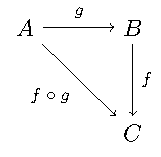
\includegraphics[width=.9\linewidth]{./function-composition.png}

\begin{block}{(2.8) composition is associative : $(f \circ g) \circ h = f \circ (g \circ h)$}
Similar to $(a + b) + c = a + (b + c)$

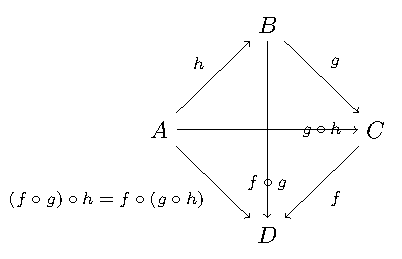
\includegraphics[width=.9\linewidth]{./function-composition-associative.png}

\rule{\linewidth}{0.5pt}
\end{block}
\end{frame}
\begin{frame}[fragile,label=sec-3]{2.4  (2.9) identity function(s) : $id \hspace{0.25em} x = x$}
 \url{http://hackage.haskell.org/package/base-4.7.0.1/docs/src/GHC-Base.html#id}

\begin{verbatim}
id   :: a -> a
id x = x
\end{verbatim}

\texttt{id} does not lose any information

\begin{block}{(2.10) \texttt{id} is the \emph{unit} of composition : $f \circ id = id \circ f = f$}
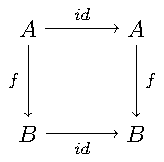
\includegraphics[width=.9\linewidth]{./function-composition-id-is-unit.png}

\rule{\linewidth}{0.5pt}
\end{block}
\end{frame}
\begin{frame}[fragile,label=sec-4]{2.5  (2.12) constant function(s) : $const \hspace{0.25em} x \hspace{0.25em} \_ =  x$}
 \url{http://hackage.haskell.org/package/base-4.7.0.1/docs/src/GHC-Base.html#const}

\begin{verbatim}
const     :: a -> b -> a
const x _ =  x
\end{verbatim}

A function that results after apply \texttt{const} to \texttt{x}

\begin{verbatim}
c' :: a -> Char
c'  = const 'c'
\end{verbatim}

loses all information (i.e., ignores its argument).

\begin{block}{(2.13) constant-fusion : $c \circ f = c$}
\begin{verbatim}
constantFusion  :: (x -> y) -> x -> Char
constantFusion f = c' . f
\end{verbatim}

The following diagram shows
\begin{itemize}
\item c' as the function (\texttt{const\_2}) that results from applying \texttt{const} (here shown as \texttt{const\_1}) to \texttt{Char}
\item \texttt{f} applied to \texttt{x} resulting in \texttt{y}
\item \texttt{const\_2} applied to \texttt{y} resulting in \texttt{Char}
\end{itemize}

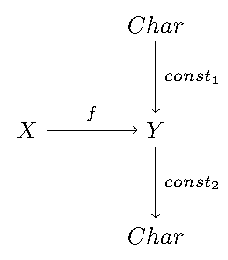
\includegraphics[width=.9\linewidth]{./constant-fusion.png}

Note
\begin{itemize}
\item input to \texttt{f} can be any type
\item result of \texttt{f} can be any type
\item ignores result of \texttt{f}
\item output of constant-fusion not (necessarily) type related to co/domain of \texttt{f}
\end{itemize}

constant-fusion example

\begin{verbatim}
c :: a -> Char
c = const 'c'

c0 = U.t "c0"
     (c'        . (+1)       $ 45)
     'c'

c1 = U.t "c1"
     (const 30  . ("foo" ++) $ "bar")
     30
\end{verbatim}

\alert{Exercise 2.1}

These two functions have the same type:

\begin{verbatim}
fc1 :: (c -> a) -> c -> b -> a
fc1 f c = f . const c

fc2 :: (c -> a) -> c -> b -> a
fc2 f c = const (f c)
\end{verbatim}

Regarding the functions that result from applying \texttt{fc1} and \texttt{fc2} to \texttt{f} and \texttt{c}

\begin{itemize}
\item 1st arg: domain and argument to \texttt{f}
\item 2nd arg: ignored
\item output: codomain and result of \texttt{f}
\end{itemize}

From the outside there is no difference.

On the inside

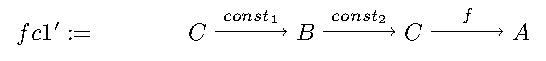
\includegraphics[width=.9\linewidth]{./e2-1a.png}

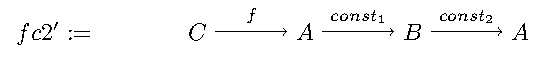
\includegraphics[width=.9\linewidth]{./e2-1b.png}

\begin{itemize}
\item fc1' first "remembers" the first arg, then ignores \texttt{b}, then applies \texttt{f} to the remembered value.
\item fc2' first applies \texttt{f} to the first arg and "remembers" the result, that is returned after ignoring \texttt{b}.
\end{itemize}

\rule{\linewidth}{0.5pt}
\end{block}
\end{frame}
\begin{frame}[fragile,label=sec-5]{2.6 monics (one-to-one/injective) and epics (onto/surjective)}
 Identity and constant functions are limit points with respect to information preservation
\begin{itemize}
\item identity preserves all information
\item constant loses all information
\end{itemize}

All other functions lose some information (regarded as unneeded in context).

Functional programming: art of transforming or losing information in a controlled manner to fit context.

Functions lose information when
\begin{itemize}
\item give same output for two or more inputs (e.g., constant function)
\item only use one value of codomain (e.g., constant function)
\end{itemize}

\url{http://en.wikipedia.org/wiki/Bijection,_injection_and_surjection}

Injective functions (aka "one-to-one", "monic") do not lose information
\begin{itemize}
\item each element of domain maps to unique element of codomain
\item (but not all elements of codomain are necessarily mapped to)
\item Categorical generalization of injective functions called "monic"
\begin{itemize}
\item \url{http://en.wikipedia.org/wiki/Monic_morphism}
\end{itemize}
\end{itemize}

Surjective functions (aka "onto", "epic") do not lose information
\begin{itemize}
\item all elements of codomain are mapped to
\item Categorical generalization of surjective functions call "epic" (but converse is not true in all categories)
\begin{itemize}
\item \url{http://en.wikipedia.org/wiki/Epimorphism}
\end{itemize}
\end{itemize}

\alert{Exercise 2.2}

Under what circumstances is a constant function epic?

\begin{verbatim}
data Single = Single deriving Show

epicConstantFunction :: b -> Single
epicConstantFunction = const Single
\end{verbatim}

\rule{\linewidth}{0.5pt}
\end{frame}
\begin{frame}[fragile,label=sec-6]{2.7 (2.16) isomorphisms : $f \circ f^{\circ} = id_b \wedge f^{\circ} \circ f = id_a$}
 A \emph{isomorphic} function (aka \emph{bijective}) is one-to-one (monic) and onto (epic).

\url{http://en.wikipedia.org/wiki/Isomorphism}

Given $f : A \rightarrow B$,
$f$ has \emph{inverse}
$f^{\circ} : B \rightarrow A$,
such that 2.16 (above) holds.

Isomorphisms are important because they convert between "formats"
without losing information, although the data adopts a different
“shape” in each of them.

"A is isomorphic to B" is written: $A \cong B$.

Isomorphic data domains are regarded as "abstractly" the same.

\alert{example}

\url{http://hackage.haskell.org/package/base-4.7.0.1/docs/Prelude.html#t:Enum}

\begin{verbatim}
data Weekday = Sunday | Monday | Tuesday | Wednesday | Thursday | Friday | Saturday
             deriving (Enum, Eq, Ord, Show)

data Seven   = One    | Two    | Three   | Four      | Five     | Six    | Seven
             deriving (Enum, Eq, Ord, Show)

transform :: (Enum a, Ord a, Enum b, Ord b) => a -> b
transform = toEnum . fromEnum

i0 = U.t "i0"
     (transform Tuesday)
     Three

i1 = U.t "i1"
     (transform Three)
     Tuesday

transform2 :: (Enum a, Ord a) => Int -> a
transform2 = toEnum . (`rem` 7)

i2 = U.t "i2"
     (transform2 15)
     Two

i3 = U.t "i3"
     (transform2 15)
     Monday
\end{verbatim}

Constants, identities, epics, monics and isos are \alert{closed under
composition} (e.g., the composition of two epics is epic).

\rule{\linewidth}{0.5pt}
\end{frame}
\begin{frame}[fragile,label=sec-7]{2.8 products --- gluing functions which do not compose}
 \begin{block}{(2.18) pair def : $\langle f,g \rangle c = (f \hspace{0.25em} c, g \hspace{0.25em} c)$}
$\langle f,g \rangle : C \rightarrow A \times B$

Not every two functions can be composed, e.g., $f : C \rightarrow A$
and $g : C \rightarrow B$ (because domain of one is not codomain of other).

But, since $f$ and $g$ share the same domain $C$, their outputs can be paired (aka "split")

\url{http://www.haskell.org/ghc/docs/7.4.1/html/libraries/ghc-prim-0.2.0.0/src/GHC-Tuple.html#\%28\%2C\%29}

\url{https://hackage.haskell.org/package/base-4.4.0.0/docs/src/Data-Tuple.html}

\begin{verbatim}
-- cartesian product of types
pair :: (c -> a) -> (c -> b) -> c -> (a,b)
pair f g c = (f c, g c)

split = pair -- aka

p0 = U.tt "p0"
     [ (    transform `pair`     show) Sunday
     , (arr transform  &&&   arr show) Sunday
     ]
     (One, "Sunday")

-- cartesian product of elements
p1 = U.t "p1"
     [ (b,c) | b <- [Sunday, Monday, Tuesday], c <- [One, Two]]
     [(Sunday,One),(Sunday,Two),(Monday,One),(Monday,Two),(Tuesday,One),(Tuesday,Two)]
\end{verbatim}
\end{block}

\begin{block}{(2.20) $\times$-cancellation : \texttt{fst} / \texttt{snd} projections}
\begin{verbatim}
p2 = U.t "p2" (fst (1,2)) 1
p3 = U.t "p3" (snd (1,2)) 2
\end{verbatim}

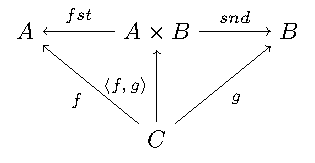
\includegraphics[width=.9\linewidth]{./pair.png}
\end{block}

\begin{block}{(2.22) $\times$ of two functions def : $f \times g = \langle f \circ fst, g \circ snd \rangle$}
Use when domains do not coincide.

\begin{verbatim}
product :: (c -> a) -> (d -> b) -> (c,d) -> (a,b)
product f g = pair (f . fst) (g . snd)

p4 = U.tt "p4"
     [ ((    (*2) `PDBC.product`     (++"bar"))   (2,"foo"))
     , ((arr (*2) ***            arr (++"bar"))   (2,"foo"))
     ]
     (4, "foobar")
\end{verbatim}

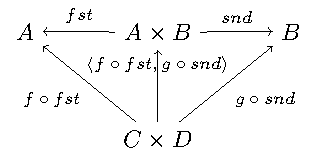
\includegraphics[width=.9\linewidth]{./product.png}
\end{block}

\begin{block}{(2.24) $\times$-fusion : $\langle g,h \rangle \circ f = \langle g \circ f, h \circ f \rangle$}
Pair/split is right-distributive with respect to composition

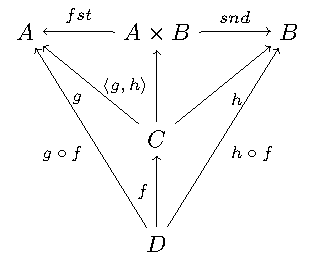
\includegraphics[width=.9\linewidth]{./product-fusion.png}

\begin{verbatim}
p5 = U.tt "p5"
     [ (pair (*2) show . digitToInt)                  '3'
     ,  pair ((*2) . digitToInt) (show . digitToInt)  '3'
     ]
     (6,"3")
\end{verbatim}

Left-distributivity does not hold.
\end{block}

\begin{block}{(2.25) $\times$-absorption : $(i \times j) \circ \langle g,h \rangle = \langle i \circ g,j \circ h \rangle$}
pair absorbs $\times$ as a kind of fusion -- a consequence for $\times$-fusion and $\times$-cancellation.

For $f \circ \langle g,h \rangle$ when $f = i \times j$

\begin{center}
\begin{tabular}{llll}
 &  &  & $(i \times j) \circ \langle g,h \rangle$\\
(2.22) & product of 2 funs def & = & $\langle i \circ fst, j \circ snd \rangle \circ \langle g,h \rangle$\\
(2.24) & $\times$-fusion & = & $\langle (i \circ fst) \circ \langle g, h \rangle,(j \circ snd) \circ \langle g,h \rangle \rangle$\\
(2.8) & associative composition & = & $\langle i \circ (fst \circ \langle g, h \rangle),j \circ (snd \circ \langle g,h \rangle) \rangle$\\
(2.20) & $\times$-cancellation & = & $\langle i \circ g,j \circ h \rangle$\\
\end{tabular}
\end{center}

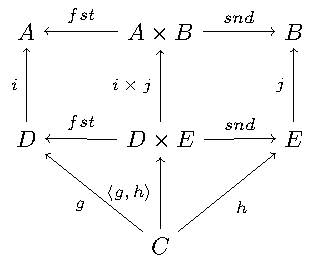
\includegraphics[width=.9\linewidth]{./product-absorption.png}

\begin{verbatim}
-- non-optimized version
pcp                        :: (d -> a) -> (e -> b) -> (c -> d) -> (c -> e) -> c -> (a, b)
pcp                i j g h = PDBC.product i j . pair g h

-- optimized version via 2.20
productComposePair         :: (d -> a) -> (e -> b) -> (c -> d) -> (c -> e) -> c -> (a, b)
productComposePair i j g h = pair (i . g) (j . h)

p6 = U.tt "p6"
     [ pcp                show read (*2) show   4
     , productComposePair show read (*2) show   4
     ]
     ("8",4)
\end{verbatim}
\end{block}

\begin{block}{(2.26) : $i \circ fst = fst \circ (i \times j)$}
\end{block}
\begin{block}{(2.27) : $j \circ snd = snd \circ (i \times j)$}
\begin{itemize}
\item (2.26) : given $D \times E$ no need to evaluate $j$
\item (2.27) : given $D \times E$ no need to evaluate $i$
\end{itemize}

\begin{verbatim}
p7 = U.tt "p7"
     [ (fst . (PDBC.product show show))        (3, 4)
     , show $ fst                              (3, 4) -- optimized via 2.26
     ]
     "3"
\end{verbatim}
\end{block}

\begin{block}{(2.28) $\times$-functor : $(g \circ h) \times (i \circ j) = (g \times i) \circ (h \times j)$}
\begin{verbatim}
productFunctorLeft  :: (e -> a) -> (c -> e) -> (f -> b) -> (d -> f) -> (c, d) -> (a, b)
productFunctorLeft  g h i j = PDBC.product (g . h) (i . j)

productFunctorRight :: (e -> a) -> (c -> e) -> (f -> b) -> (d -> f) -> (c, d) -> (a, b)
productFunctorRight g h i j = PDBC.product g i . PDBC.product h j

p8 = U.tt "p8"
     [ ((productFunctorLeft  (+2) (+4) (+6.0) (+8.0))::(Int,Double)->(Int,Double))        (1,100.0)
     , ((productFunctorRight (+2) (+4) (+6.0) (+8.0))::(Int,Double)->(Int,Double))        (1,100.0)
     ]
     (7,114.0)
\end{verbatim}
\end{block}

\begin{block}{(2.29) $\times$-functor-id : $id_A \times id_B = id_{A \times B}$}
\begin{verbatim}
p9 = U.tt "p9"
     [ PDBC.product id id    ("x", 'y')
     , id                    ("x", 'y')
     ]
     ("x", 'y')
\end{verbatim}
\end{block}

\begin{block}{(2.30) $\times$-reflexion : $\langle fst,snd \rangle = id_{A \times B}$}
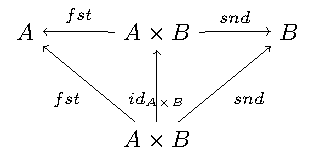
\includegraphics[width=.9\linewidth]{./product-reflexion.png}

\begin{verbatim}
p10 = U.tt "p10"
     [ pair fst snd     ("x", 'y')
     , id               ("x", 'y')
     ]
     ("x", 'y')
\end{verbatim}
\end{block}

\begin{block}{(2.31) $\times$ is commutative : $A \times B \cong B \times A$}
$\langle snd,fst \rangle = swap$

\begin{verbatim}
swap0    :: (a,b) -> (b,a)
swap0 ab = (,) (snd ab) (fst ab)
-- swap0 (a,b) = (b,a)
\end{verbatim}

Isomorphic:

\begin{center}
\begin{tabular}{llll}
 &  &  & $swap \circ swap$\\
 & def swap & = & $\langle snd,fst \rangle \circ swap$\\
(2.24) & $\times$-fusion & = & $\langle snd \circ swap,fst \circ swap \rangle$\\
 & def swap & = & $\langle snd \circ \langle snd,fst \rangle, fst \circ \langle snd,fst \rangle$\\
(2.20) & $\times$-cancellation & = & $\langle fst,snd \rangle$\\
(2.30) & $\times$-reflexion & = & $id$\\
\end{tabular}
\end{center}

Therefore, no information is lost (or gained) when swapping fields in record datatypes.
\end{block}

\begin{block}{(2.32) $\times$ is associative : $A \times (B \times C) \cong (A \times B) \times C$}
$assocl = \langle \langle fst, fst \circ snd \rangle, snd \circ snd \rangle$ \\
$assocr = \langle fst \circ fst, \langle snd \circ fst, snd \rangle \rangle$

\begin{verbatim}
assocl              :: (a, (b,c)) -> ((a,b),c)
-- assocl (a,(b,c)) = ((a,b),c)
assocl              = pair   (pair fst (fst . snd))  (snd . snd)

assocr              :: ((a,b),c) -> (a,(b,c))
-- assocr ((a,b),c) = (a,(b,c))
assocr              = pair   (fst . fst)             (pair (snd . fst) snd)  -- (2.33)
\end{verbatim}

\begin{verbatim}
p11 = U.tt "p11"
      [ (assocr . assocl) ('a', ('b', 'c'))
      , id                ('a', ('b', 'c'))
      ]
      ('a', ('b', 'c'))
\end{verbatim}

\alert{Exercise 2.3}

\begin{center}
\begin{tabular}{llll}
 &  & = & $(assocr \circ assocl) (a, (b, c))$\\
 & assocl def & = & $(assocr \circ \langle \langle fst      ,  fst \circ snd \rangle            ,  snd \circ snd \rangle) (a, (b, c))$\\
(2.18) & pair def & = & $(assocr \circ (       \langle fst      ,  fst \circ snd \rangle (a, (b, c)), (snd \circ snd) (a, (b, c))   )$\\
(2.20) x 2 & $\times$-cancellation & = & $(assocr \circ (       \langle fst      ,  fst \circ snd \rangle (a, (b, c)),                         c     )$\\
(2.18) & pair def & = & $(assocr \circ (        (fst (a, (b, c)), (fst \circ snd) (a, (b, c)) ),                              c     )$\\
(2.20) x 3 & $\times$-cancellation & = & $(assocr \circ (        (     a         ,                      b      ),                              c     )$\\
 &  & = & \ldots{}\\
 &  & = & $(a, (b, c))$\\
\end{tabular}
\end{center}

\alert{Exercise 2.4}

Use (2.22) (product of two functions) to prove (2.28) ($\times$-functor) and (2.29) ($\times$-functor-id).

Prove (2.28):

\begin{center}
\begin{tabular}{rlll}
 &  &  & $((g \circ h) \times (i \circ j))$\\
2.22 &  & = & $\langle (g \circ h) \circ fst, (i \circ j) \circ snd \rangle$\\
 &  &  & TODO \ldots{}\\
\end{tabular}
\end{center}


\rule{\linewidth}{0.5pt}
\end{block}
\end{frame}
\begin{frame}[fragile,label=sec-8]{2.9 coproducts --- gluing functions which do not compose}
 \begin{block}{(2.35) either def : $[f,g] : A + B \rightarrow C$}
\emph{coproduct} of $A$ and $B$ is \emph{disjoint union} data type that has
values "stamped" with different tags to indicate whether the value
came from $A$ or $B$.

\url{https://hackage.haskell.org/package/base-4.7.0.0/docs/src/Data-Either.html#either}

Use \texttt{Either} with \texttt{Left} / \texttt{Right} \emph{injections}.

\begin{verbatim}
either :: (a -> c) -> (b -> c) -> Either a b -> c
either f _ (Left  a) = f a
either _ g (Right b) = g b
\end{verbatim}

\begin{verbatim}
e1 = U.tt "e1"
     [ ((*11)     `PDBC.either`     (+1))   (Left   9)
     , ((*11)     `PDBC.either`     (+1))   (Right 98)
     , (arr (*11)  |||          arr (+1))   (Left   9)
     , (arr (*11)  |||          arr (+1))   (Right 98)
     ]
     99
\end{verbatim}

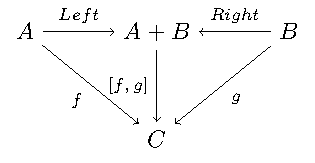
\includegraphics[width=.9\linewidth]{./either.png}

\emph{product} and \emph{coproduct} are \emph{dual} mathematical constructs.  Duality
means that everythings said about product $A \times B$ can be rephrased to
coproduct $A + B$.

The sum of two functions \texttt{f + g} is the dual of the product of two functions \texttt{f × g} :
\end{block}

\begin{block}{(2.37) $+$ of two functions def : $f + g = [Left \circ f, Right \circ g]$}
\begin{verbatim}
sum :: (a -> c) -> (b -> d) -> Either a b -> Either c d
sum f g  = PDBC.either (Left . f) (Right . g)
\end{verbatim}

\begin{verbatim}
su1 = U.tt "su1"
      [ (    (*11) `PDBC.sum`     (+1))   (Left 9)
      , (arr (*11)  +++       arr (+1))   (Left 9)
      ]
      (Left 99)
\end{verbatim}
\end{block}

\begin{block}{(2.38) $+$-cancellation : $[g,h] \circ Left = g$, $[g,h] \circ Right = h$}
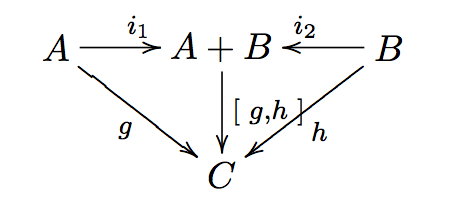
\includegraphics[width=.9\linewidth]{./sum-cancellation.png}

\begin{verbatim}
sc1 = U.tt "sc1"
      [ (PDBC.either (+10) (*10) . Left)  10
      ,              (+10)                10
      ]
      20
sc2 = U.tt "sc2"
      [ (PDBC.either (+10) (*10) . Right) 10
      ,                    (*10)          10
      ]
      100
\end{verbatim}
\end{block}

\begin{block}{(2.39) $+$-reflexion : $[ Left, Right ] = id_{A + B}$}
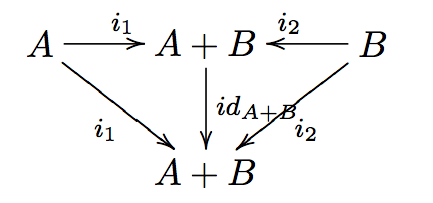
\includegraphics[width=.9\linewidth]{./sum-reflexion.png}

\begin{verbatim}
sr1 = U.tt "sr1"
      [ (PDBC.either Left Right    (Left   10)
                 :: (Show a, Num a, Show b, Num b) => Either a b)
      , id                         (Left   10)
      ]
      (Left 10)

sr2 = U.tt "sr2"
      [ (PDBC.either Left Right    (Right 100)
                 :: (Show a, Num a, Show b, Num b) => Either a b)
      , id                         (Right 100)
      ]
      (Right 100)
\end{verbatim}
\end{block}

\begin{block}{(2.40) $+$-fusion : $f \circ [ g , h ] = [ f \circ g , f \circ h ]$}
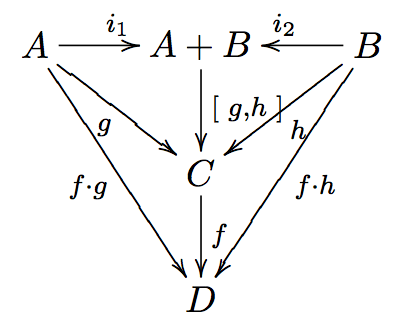
\includegraphics[width=.9\linewidth]{./sum-fusion.png}

\begin{verbatim}
sumFusionLeft, sumFusionRight :: (c -> d) -> (a -> c) -> (b -> c) -> Either a b -> d
sumFusionLeft  f g h = f . (PDBC.either g h)
sumFusionRight f g h = PDBC.either (f . g) (f . h)
\end{verbatim}
\end{block}

\begin{block}{(2.41) $+$-absorption : $[ g , h ] \circ ( i + j ) = [ g \circ i, h \circ j ]$}
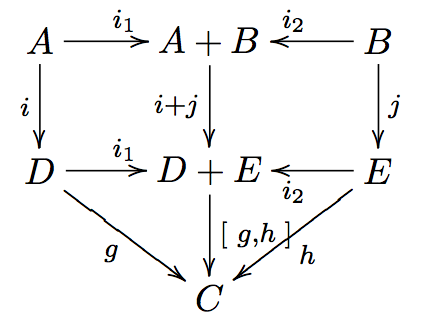
\includegraphics[width=.9\linewidth]{./sum-absorption.png}

\begin{verbatim}
sumAbsorptionLeft, sumAbsorptionRight :: (d -> c) -> (e -> c) -> (a -> d) -> (b -> e) -> Either a b -> c
sumAbsorptionLeft  g h i j = (PDBC.either g h) . (PDBC.sum i j)
sumAbsorptionRight g h i j = PDBC.either (g . i) (h . j)
\end{verbatim}
\end{block}

\begin{block}{(2.42) $+$-functor : $(g \circ h) + (i \circ j) = (g + i) \circ (h + j)$}
\begin{figure}[htb]
\centering
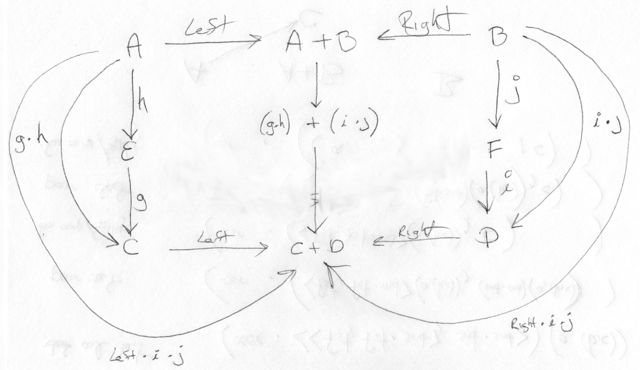
\includegraphics[width=.9\linewidth]{./sum-functor-1m.jpg}
\caption{left}
\end{figure}

\begin{figure}[htb]
\centering
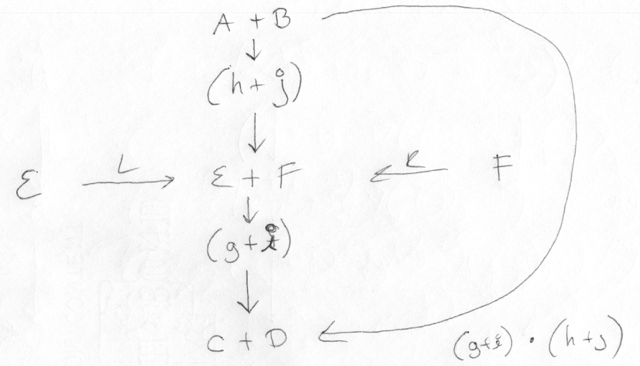
\includegraphics[width=.9\linewidth]{./sum-functor-2m.png}
\caption{right}
\end{figure}

\begin{verbatim}
sumFunctorLeft, sumFunctorRight :: (e -> c) -> (a -> e) -> (f -> d) -> (b -> f) -> Either a b -> Either c d
sumFunctorLeft  g h i j = PDBC.sum (g . h) (i . j)
sumFunctorRight g h i j = (PDBC.sum g i) . (PDBC.sum h j)
\end{verbatim}
\end{block}

\begin{block}{(2.43) $+$-functor-id : $id_A + id_B = id_{A+B}$}
TODO : diagram

\begin{verbatim}
sumFunctorIdLeft, sumFunctorIdRight :: Either a b -> Either a b
sumFunctorIdLeft  = PDBC.sum id id
sumFunctorIdRight = id
\end{verbatim}

\alert{Exercise 2.5}  TODO

\alert{Exercise 2.6}  TODO

\rule{\linewidth}{0.5pt}
\end{block}
\end{frame}
\begin{frame}[fragile,label=sec-9]{2.10 mixing products and coproducts}
 \begin{block}{(2.47) pair/either exchange : $[ \langle f , g \rangle , \langle h , k \rangle ] = \langle [ f , h ], [ g , k ] \rangle$}
\begin{verbatim}
{-
peExchangeLeft, peExchangeRight :: (a -> a') -> (a -> b') -> (b -> a') -> (b -> b') -> Either a b -> (a', b')
-}
peExchangeLeft, peExchangeRight :: (a -> b)  -> (a -> d)  -> (c -> b)  -> (c -> d)  -> Either a c -> (b,  d)

peExchangeLeft  f g h k = PDBC.either (pair        f g) (pair        h k)
peExchangeRight f g h k = pair        (PDBC.either f h) (PDBC.either g k)
\end{verbatim}
\end{block}

\begin{block}{(2.49) undistr def : $undistr = [ id \times first , id \times snd ]$}
\begin{verbatim}
undistr :: Either (a,b) (a,c) -> (a, Either b c)
undistr  = PDBC.either (PDBC.product id Left) (PDBC.product id Right)
\end{verbatim}

undistr shows:
\end{block}

\begin{block}{(2.50) isomorphism: product distributes through coproduct : $(A \times B) + (A \times C) \cong A \times (B + C)$}
\end{block}

\begin{block}{motivation for functors}
\begin{center}
\begin{tabular}{llll}
 & given &  & $f : A \rightarrow E$\\
 & given &  & $g : B \rightarrow E$\\
 & given &  & $h : C \rightarrow F$\\
(2.37) & $+$ of two functions def & = & $g + h : B + C \rightarrow E + F$\\
(2.22) & $\times$ of two functions def & = & $f \times (g + h) : A \times (B + C) \rightarrow D \times (E + F)$\\
\end{tabular}
\end{center}

Preserves shape, but changes internal element types.

Combination of products and sums of functions have same shape as the
expressions that denote their domain and range.

Now abstract

\begin{itemize}
\item left of (2.50) as : def G$(a,b,c) = (a \times b) + (a \times c)$
\item right of (2.50) as : def F$(a,b,c) = a \times (b + c)$
\item where $a$, $b$, $c$ denote types
\end{itemize}

then, with specific types and functions:

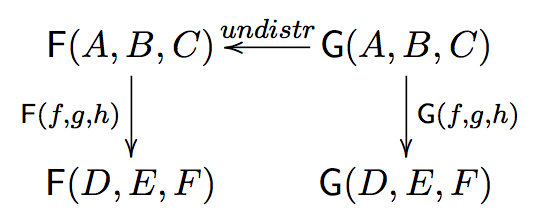
\includegraphics[width=.9\linewidth]{./F-G-undistr.png}

which instantiates to:

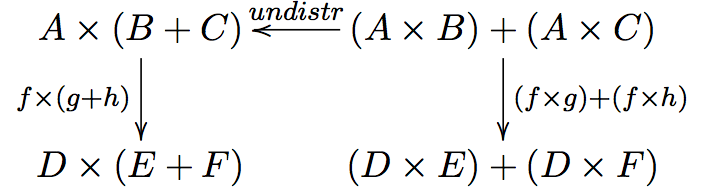
\includegraphics[width=.9\linewidth]{./F-G-undistr-instantiated.png}

\alert{Exercise 2.7} TODO

\alert{Exercise 2.8} TODO

\alert{Exercise 2.9} TODO

\rule{\linewidth}{0.5pt}

\begin{verbatim}
main =
    T.runTestTT $ T.TestList $ c0 ++ c1 ++
                               i0 ++ i1 ++ i2 ++ i3 ++
                               p0 ++ p1 ++ p2 ++ p3 ++ p4 ++ p5 ++ p6 ++ p7 ++ p8 ++ p9 ++ p10 ++ p11 ++
                               e1 ++
                               su1 ++
                               sc1 ++ sc2 ++ sr1 ++ sr2
\end{verbatim}
\end{block}
\end{frame}
\end{document}
